% =====================================================================
%  Chapter: Mechanics as the Statistical Mechanics of Pure States
%
%  Everything above \begin{document} is a minimal preamble so that the
%  file compiles on its own.  To use the chapter inside the book, copy
%  the macros and theorem environments into the book preamble and
%  \input the text between  %%% BEGIN CHAPTER  and  %%% END CHAPTER.
% =====================================================================
\documentclass[11pt,a4paper]{book}

\usepackage[T1]{fontenc}
\usepackage[utf8]{inputenc}
\usepackage{lmodern}
\usepackage[margin=2.8cm]{geometry}
\usepackage{amsmath,amssymb,amsthm,mathtools,bm}
\usepackage{booktabs,enumitem}
\usepackage{tikz}
\usepackage[hidelinks]{hyperref}

% ---------- macros ----------
\newcommand{\dd}{\mathrm{d}}
\newcommand{\kB}{k_{\mathrm B}}
\newcommand{\R}{\mathbb{R}}
\newcommand{\Ave}[1]{\left\langle #1\right\rangle}
\newcommand{\PB}[2]{\{#1,#2\}}
\newcommand{\eu}{\mathrm{e}}
\DeclareMathOperator{\Var}{Var}
\DeclareMathOperator{\Cov}{Cov}
\DeclareMathOperator{\supp}{supp}
\DeclareMathOperator{\Tr}{Tr}
\DeclareMathOperator{\KL}{D}

% ---------- theorem-like environments ----------
\theoremstyle{plain}
\newtheorem{proposition}{Proposition}[chapter]
\theoremstyle{definition}
\newtheorem{definition}[proposition]{Definition}
\newtheorem{example}[proposition]{Example}
\newtheorem{exercise}{Exercise}[chapter]
\theoremstyle{remark}
\newtheorem{remark}[proposition]{Remark}

\begin{document}

%%% BEGIN CHAPTER
\chapter{Mechanics as the Statistical Mechanics of Pure States}
\label{ch:pure-mixed}

\section{Two theories or one?}

Textbooks present mechanics and statistical mechanics as two different theories. Mechanics deals with a few bodies and gives their trajectories. Statistical mechanics deals with an enormous number of particles, in the thermodynamic limit an infinite number, and gives probability distributions instead of trajectories. The dividing line is drawn by the number of particles.

This chapter argues that the dividing line is drawn in the wrong place. The number of particles is a practical circumstance that usually accompanies the choice between the two descriptions, but it is not what distinguishes them. Three examples make the point.

\begin{itemize}[nosep]
\item A single harmonic oscillator in thermal contact with a reservoir is described by the Boltzmann distribution $\propto\eu^{-H/\kB T}$. Here $N=1$, and the description is statistical.
\item Maxwell's distribution of velocities is, before it is a statement about a gas, a statement about \emph{one} molecule: it gives the probability that a molecule drawn from the gas has a given velocity.
\item The Solar System, with $N\approx 10$ bodies of interest, is a mechanical system. Yet its long-term prediction is carried out with probability densities of initial conditions, and a molecular-dynamics simulation with $10^5$ atoms is a purely mechanical calculation.
\end{itemize}

What distinguishes the two descriptions is the \emph{kind of state} they admit. Mechanics assigns to a system a point of phase space. Statistical mechanics assigns a probability distribution on phase space. A point is a very special distribution: all of the probability sits at one place. Seen this way, mechanics is not a rival of statistical mechanics but the part of it that deals with states of the special form $\delta(z-z_0)$.

\begin{center}
\fbox{\parbox{0.88\linewidth}{\textbf{Thesis.} Mechanics and statistical mechanics are one theory with one phase space, one kind of observable and one law of motion. They differ only in which states are admitted: \emph{pure states} (points of phase space) in mechanics, and arbitrary \emph{mixed states} (probability distributions) in statistical mechanics. Mechanics is the pure-state sector.}}
\end{center}

\paragraph{Two claims, to be kept apart.} The thesis contains two claims of different character.

\begin{description}[nosep,leftmargin=1.5em]
\item[(M)] A mathematical claim. The set of pure states is closed under the dynamics, and on this set the dynamics of statistical mechanics (the Liouville equation) is exactly the dynamics of mechanics (Hamilton's equations). This is a theorem, and it is true whatever one thinks probability means.
\item[(B)] An interpretive claim. A mixed state is a state of \emph{knowledge}: a probability distribution quantifies what an observer knows about a system, and the difference between pure and mixed is the difference between complete and incomplete knowledge. This is the Bayesian reading, and it is a position one may or may not adopt; Section~\ref{sec:objections} discusses what it costs and what it buys.
\end{description}

Sections~\ref{sec:states} and~\ref{sec:dynamics} establish (M). Sections~\ref{sec:bayes} and~\ref{sec:entropy} develop (B) and its consequences for entropy and irreversibility. Section~\ref{sec:examples} works out examples, among them the transition between the statistical and the mechanical regime. Section~\ref{sec:subsystems} looks at subsystems and at the quantum case.

% ---------------------------------------------------------------------
\section{States: pure and mixed}
\label{sec:states}

\subsection{Phase space and observables}

Consider a Hamiltonian system with $n$ degrees of freedom. Its phase space is $\Gamma=\R^{2n}$ with canonical coordinates $z=(q_1,\dots,q_n,p_1,\dots,p_n)$ and with the Liouville measure $\dd z=\dd^n q\,\dd^n p$. (Everything below holds on a general symplectic manifold; the coordinates keep the formulas short.) An \emph{observable} is a real function $A:\Gamma\to\R$. The Poisson bracket is
\begin{equation}
\PB{A}{B}=\sum_{i=1}^{n}\left(\frac{\partial A}{\partial q_i}\frac{\partial B}{\partial p_i}-\frac{\partial A}{\partial p_i}\frac{\partial B}{\partial q_i}\right),
\end{equation}
and the dynamics is generated by a Hamiltonian $H$, so that Hamilton's equations read $\dot z=\PB{z}{H}$, that is,
$\dot q_i=\partial H/\partial p_i$ and $\dot p_i=-\partial H/\partial q_i$.

\subsection{States as probability measures}

\begin{definition}[state]
A \emph{state} is a probability measure $\mu$ on $\Gamma$. The expectation of an observable $A$ in the state $\mu$ is $\Ave{A}_\mu=\int_\Gamma A\,\dd\mu$ and its variance is $\Var_\mu A=\Ave{A^2}_\mu-\Ave{A}_\mu^2$. If $\mu$ has a density, $\dd\mu=\rho\,\dd z$ with $\rho\ge0$ and $\int\rho\,\dd z=1$, we speak of the density of the state.
\end{definition}

The word \emph{measure} instead of \emph{density} is not pedantry. The states of mechanics, the points, have no density in the ordinary sense. The Dirac measure $\delta_{z_0}$, defined by $\delta_{z_0}(B)=1$ if $z_0\in B$ and $0$ otherwise, is a perfectly good probability measure; as a ``density'' it is the distribution $\rho(z)=\delta(z-z_0)$. A framework restricted to ordinary densities would exclude the very states we want to include.

The set $\mathcal S$ of all states is \emph{convex}: if $\mu_1,\mu_2\in\mathcal S$ and $0\le\lambda\le1$, then $\lambda\mu_1+(1-\lambda)\mu_2\in\mathcal S$. This is the formal counterpart of mixing two preparations: with probability $\lambda$ the system is prepared as in $\mu_1$ and otherwise as in $\mu_2$.

\begin{definition}[pure and mixed states]
A state is \emph{pure} if it is a Dirac measure $\delta_{z_0}$, and \emph{mixed} otherwise.
\end{definition}

The definition singles out points of phase space, as it should. The next proposition shows that it also singles out exactly the states one would call ``states of complete knowledge'' by any of three independent criteria.

\begin{proposition}[characterizations of pure states]\label{prop:pure}
For a state $\mu$ on $\Gamma$ the following are equivalent:
\begin{enumerate}[label=(\alph*),nosep]
\item $\mu=\delta_{z_0}$ for some $z_0\in\Gamma$;
\item $\mu$ is dispersion-free: $\Var_\mu A=0$ for every bounded continuous observable $A$;
\item $\mu$ is multiplicative: $\Ave{AB}_\mu=\Ave{A}_\mu\Ave{B}_\mu$ for all bounded continuous $A,B$;
\item $\mu$ is an extreme point of $\mathcal S$: it cannot be written as $\lambda\mu_1+(1-\lambda)\mu_2$ with $\mu_1\neq\mu_2$ and $0<\lambda<1$.
\end{enumerate}
\end{proposition}

\begin{proof}
(a)$\Rightarrow$(c): $\Ave{AB}_{\delta_{z_0}}=A(z_0)B(z_0)$. (c)$\Rightarrow$(b): put $B=A$.

(b)$\Rightarrow$(a): zero variance means $A=\Ave{A}_\mu$ $\mu$-almost everywhere. Apply this to the bounded continuous functions $A_i=\arctan z_i$, $i=1,\dots,2n$. Each coordinate is then almost surely constant, so $\mu$ is concentrated at a single point.

(a)$\Rightarrow$(d): suppose $\delta_{z_0}=\lambda\mu_1+(1-\lambda)\mu_2$ with $0<\lambda<1$. Then $\lambda\mu_1(\Gamma\setminus\{z_0\})\le\delta_{z_0}(\Gamma\setminus\{z_0\})=0$, so $\mu_1=\delta_{z_0}$, and likewise $\mu_2=\delta_{z_0}$.

(d)$\Rightarrow$(a): if $\mu$ is not a Dirac measure, its support contains two distinct points. Choose disjoint open neighbourhoods $U,V$ of them; both have positive measure by definition of the support. With $p=\mu(U)\in(0,1)$ we can write $\mu=p\,\mu(\cdot\,|\,U)+(1-p)\,\mu(\cdot\,|\,\Gamma\setminus U)$, a nontrivial mixture of two different states, since they are concentrated on disjoint sets. So $\mu$ is not extreme.
\end{proof}

The three criteria are three ways of saying that there is no ignorance. Criterion (b) says that every observable has a sharp value. Criterion (c) says that the state carries no correlations beyond the values themselves: expectations factorize. Criterion (d) says that the state cannot be interpreted as a mixture of preparations; it is irreducible. In algebraic language, (c) says that a pure state is a \emph{character} of the commutative algebra of observables, that is, evaluation at a point.

\begin{remark}[unique decomposition]
Every state is a mixture of pure states, $\mu=\int\delta_z\,\dd\mu(z)$, and the decomposition is \emph{unique}: the set $\mathcal S$ is a simplex. Classically, a mixed state is therefore \emph{one and only one} distribution over points. This is what makes the ignorance reading of mixedness unproblematic here. In quantum theory the analogous statement fails, as Section~\ref{sec:quantum} explains.
\end{remark}

\begin{table}[t]
\centering
\renewcommand{\arraystretch}{1.25}
\begin{tabular}{@{}p{2.7cm}p{5.4cm}p{6.1cm}@{}}
\toprule
 & Pure state (mechanics) & Mixed state (statistical mechanics)\\
\midrule
State & point $z_0\in\Gamma$, $\ \mu=\delta_{z_0}$ & probability measure $\mu$ on $\Gamma$\\
Observable $A$ & has the value $A(z_0)$ & has expectation $\int A\,\dd\mu$ and a spread\\
Law of motion & Hamilton's equations & Liouville equation\\
Information & complete (infinite) & incomplete (finite)\\
Gibbs entropy & $-\infty$ & finite\\
Obtained by & no finite set of measurements & Bayesian update, maximum entropy\\
\bottomrule
\end{tabular}
\caption{The two sectors of a single theory.}
\label{tab:sectors}
\end{table}

% ---------------------------------------------------------------------
\section{Dynamics: Hamilton's equations inside the Liouville equation}
\label{sec:dynamics}

Let $\varphi_t:\Gamma\to\Gamma$ be the Hamiltonian flow, the map that takes the phase point $z$ at time $0$ to its position at time $t$. By Liouville's theorem, $\varphi_t$ preserves the measure $\dd z$, that is, the Jacobian determinant of $\varphi_t$ equals $1$.

A state is carried along by the flow: if the system is in a region $B$ at time $t$ then it was in $\varphi_{-t}(B)$ at time $0$, so
\begin{equation}
\mu_t(B)=\mu_0\bigl(\varphi_{-t}(B)\bigr),\qquad
\Ave{A}_{\mu_t}=\Ave{A\circ\varphi_t}_{\mu_0}.
\label{eq:pushforward}
\end{equation}
The second formula says that one may either evolve the state and keep the observable fixed, or keep the state fixed and evolve the observable, $A_t=A\circ\varphi_t$. The two pictures are the classical analogues of the Schr\"odinger and Heisenberg pictures. Note that $A\mapsto A\circ\varphi_t$ is \emph{linear} in $A$ even though $\varphi_t$ itself is generally a nonlinear map.

For a state with density, \eqref{eq:pushforward} and the invariance of $\dd z$ give $\rho_t(\varphi_t(z))=\rho_0(z)$. Differentiating along the flow, $\partial_t\rho+\PB{\rho}{H}=0$, that is, the \emph{Liouville equation}
\begin{equation}
\frac{\partial\rho}{\partial t}=\PB{H}{\rho}.
\label{eq:liouville}
\end{equation}

\begin{proposition}[pure states stay pure]\label{prop:pure-stays-pure}
If $\mu_0=\delta_{z_0}$ then $\mu_t=\delta_{\varphi_t(z_0)}$.
\end{proposition}

\begin{proof}
By \eqref{eq:pushforward}, $\Ave{A}_{\mu_t}=\Ave{A\circ\varphi_t}_{\delta_{z_0}}=A(\varphi_t(z_0))$ for every observable $A$.
\end{proof}

In the language of densities, the solution of \eqref{eq:liouville} with initial condition $\rho_0=\delta(z-z_0)$ is $\rho_t(z)=\delta\bigl(\varphi_{-t}(z)-z_0\bigr)=\delta\bigl(z-\varphi_t(z_0)\bigr)$, where the Jacobian that would normally appear in a change of argument of the $\delta$-function equals $1$ by Liouville's theorem. The curve $t\mapsto\varphi_t(z_0)$ is the solution of Hamilton's equations. In the terminology of partial differential equations, Hamilton's equations are the \emph{characteristics} of the Liouville equation.

This proves claim (M). The set of pure states, which is a copy of $\Gamma$, is invariant under the Liouville dynamics, and the restriction of the dynamics to it is mechanics. Mechanics is a closed subtheory of statistical mechanics.

Two comments deserve to be made explicit.

\paragraph{Statistical mechanics has no new law of motion.} Equation \eqref{eq:liouville} is linear, and it is solved by moving each pure component along its own trajectory and keeping its weight: $\mu_t=\int\delta_{\varphi_t(z)}\,\dd\mu_0(z)$. The components do not interact. All new content of statistical mechanics lies in the choice of the initial mixed state and in the choice of the observables one asks about, never in an additional dynamical law. This is why the equivalence of the two descriptions is not a statement about the limit of large $N$.

\paragraph{The mean of a mixed state does not follow a trajectory.} From \eqref{eq:pushforward} one gets for any observable $\frac{\dd}{\dd t}\Ave{A}_{\mu_t}=\Ave{\PB{A}{H}}_{\mu_t}$. For $A=z_i$ this gives $\frac{\dd}{\dd t}\Ave{z}=\Ave{J\nabla H}$, where $J$ is the standard symplectic matrix. For a pure state $\Ave{J\nabla H}=J\nabla H(z)$ and we recover Hamilton's equations. For a mixed state one would need $\Ave{\nabla H(z)}=\nabla H(\Ave{z})$ to conclude that the \emph{mean} moves like a mechanical trajectory.

\begin{proposition}\label{prop:mean}
$\Ave{\nabla H}_\mu=\nabla H(\Ave{z}_\mu)$ for every state $\mu$ (with finite first moments) if and only if $H$ is a polynomial of degree at most two. In that case the mean $\Ave{z}_t$ of every state obeys Hamilton's equations.
\end{proposition}

\begin{proof}
If $\nabla H$ is affine, the identity is the linearity of the expectation. Conversely, take $\mu=\lambda\delta_a+(1-\lambda)\delta_b$. The identity becomes $\lambda\nabla H(a)+(1-\lambda)\nabla H(b)=\nabla H(\lambda a+(1-\lambda)b)$ for all $a,b$ and $\lambda\in[0,1]$, which holds only if $\nabla H$ is affine.
\end{proof}

For a particle of mass $m$ in one dimension with $H=p^2/2m+V(q)$, expanding $V'$ around the mean gives
\begin{equation}
m\,\frac{\dd^2\Ave{q}}{\dd t^2}=-\Ave{V'(q)}=-V'(\Ave q)-\tfrac12V'''(\Ave q)\,\sigma_q^2-\cdots,
\qquad \sigma_q^2=\Var q.
\label{eq:meancorr}
\end{equation}
The first term is Newton's law. The remaining terms are corrections proportional to the width of the state. Mechanics is recovered when the width tends to zero, and Eq.~\eqref{eq:meancorr} measures how far a state of finite width is from it.

% ---------------------------------------------------------------------
\section{The Bayesian reading}
\label{sec:bayes}

\subsection{A state as a state of knowledge}

So far the word ``probability'' was a mathematical term. We now give it a meaning. In the Bayesian (Cox--Jaynes) view a probability is a number that quantifies the plausibility of a proposition given the information at hand. A state $\mu$ is then the compact statement of what is known about a system: $\mu(B)$ is the plausibility that the phase point lies in $B$.

The consequence for our thesis is immediate. The system is represented, in the ideal-world model of classical mechanics, by one phase point $z^*(t)$, which obeys Hamilton's equations. An observer who does not know $z^*$ exactly describes it by a mixed state; an observer who knew it exactly would describe it by $\delta_{z^*}$. The difference between pure and mixed is the difference between complete and incomplete information. It is not a difference between two kinds of physical systems, and it is certainly not a difference between small and large systems.

This is the place where the distinction between the real world and the ideal world, drawn earlier in this book, matters. The point $z^*$ is an object of the ideal world: a model element with $2n$ real numbers, each of which has infinitely many digits. Specifying $z$ to a resolution $\varepsilon$ inside a region of linear size $L$ requires about $2n\log_2(L/\varepsilon)$ bits, which diverges as $\varepsilon\to0$. No set of measurements, however large, supplies this. What the real world supplies is a finite amount of data, and finite data always produce a mixed state. \emph{The pure state is the limit of an infinite amount of information, and therefore an idealization.} Mechanics, in this reading, is not wrong; it is the ideal-world sector of a theory whose real-world states are always mixed.

\subsection{Updating}

Learning is the only operation that turns one state into another other than the dynamics. If $\rho(z)$ is the prior density and a measurement returns the datum $d$ with likelihood $\mathcal L(d\,|\,z)$, then Bayes' theorem gives the posterior
\begin{equation}
\rho(z\,|\,d)=\frac{\mathcal L(d\,|\,z)\,\rho(z)}{\int\mathcal L(d\,|\,z')\,\rho(z')\,\dd z'}.
\label{eq:bayes}
\end{equation}

\begin{example}[measuring a position]\label{ex:bayes}
Let $n=1$. The prior is Gaussian in $q$ with mean $m_0$ and variance $\sigma_0^2$, and the instrument returns $d=q+\xi$ with Gaussian error of variance $\sigma^2$. The posterior is again Gaussian, with
\begin{equation}
\frac1{\sigma_{\rm post}^2}=\frac1{\sigma_0^2}+\frac1{\sigma^2},\qquad
m_{\rm post}=\sigma_{\rm post}^2\left(\frac{m_0}{\sigma_0^2}+\frac d{\sigma^2}\right).
\end{equation}
Precisions add. After $M$ independent measurements of the same quality the variance is of order $\sigma^2/M$. It tends to zero only as $M\to\infty$, so no finite number of observations yields a pure state. The same holds for $p$.
\end{example}

Prediction is therefore a cycle. One updates the state with the data, \eqref{eq:bayes}, transports it with the dynamics, \eqref{eq:liouville}, reads off the distribution of the observable of interest, and compares with the next measurement.

\begin{remark}[there is no collapse]
The update \eqref{eq:bayes} changes the \emph{description} and leaves the system alone. Within the classical ideal-world model the true point $z^*$ is not affected by the observer learning something about it. (A real measurement may of course disturb the system through its coupling to the apparatus. That is a dynamical process in a larger Hamiltonian system, described by Eq.~\eqref{eq:liouville} on the enlarged phase space, and it must be kept distinct from the update.) The two operations have different properties: Liouville evolution is deterministic, linear and conserves the Gibbs entropy; Bayesian updating depends on the data and typically reduces the entropy of the description.
\end{remark}

\subsection{Maximum entropy: where equilibrium ensembles come from}

Often the available information is not a point measurement but a set of macroscopic data, for example the mean energy. Suppose we know the expectations $\Ave{f_k}=F_k$ of some observables $f_1,\dots,f_r$. Among all states consistent with these constraints, the Bayesian prescription is to choose the one that assumes the least beyond the data, that is, the one that maximizes the entropy (defined in Section~\ref{sec:entropy}). Varying
$S[\rho]-\kB\sum_k\lambda_k\int\rho f_k\,\dd z-\kB\lambda_0\int\rho\,\dd z$ gives $\ln(h^n\rho)=-1-\lambda_0-\sum_k\lambda_kf_k$, that is,
\begin{equation}
\rho(z)=\frac1{Z}\exp\Bigl(-\sum_{k=1}^r\lambda_kf_k(z)\Bigr),\qquad Z=\int\exp\Bigl(-\sum_k\lambda_kf_k\Bigr)\frac{\dd z}{h^n},
\label{eq:maxent}
\end{equation}
where the multipliers $\lambda_k$ are fixed by the constraints. For $f_1=H$ one obtains the canonical state $\rho=\eu^{-\beta H}/Z$, with $\beta=1/\kB T$ the multiplier of the energy constraint. Restricting instead to a shell of fixed energy gives the microcanonical state.

\begin{proposition}\label{prop:stationary}
Any state with density $\rho=g(H)$ is stationary under the dynamics.
\end{proposition}

\begin{proof}
$\partial_t\rho=\PB{H}{g(H)}=g'(H)\PB{H}{H}=0$.
\end{proof}

Equilibrium ensembles are thus particular mixed states: the states of maximal ignorance compatible with the conserved quantities one has data on. Nothing in this argument required $N$ to be large. For a single oscillator with $H=p^2/2m+m\omega^2q^2/2$ the canonical state is a Gaussian with $\Ave{q^2}=\kB T/m\omega^2$ and $\Ave{p^2}=m\kB T$.

% ---------------------------------------------------------------------
\section{Entropy, coarse graining and irreversibility}
\label{sec:entropy}

\subsection{The Gibbs entropy}

For a state with density $\rho$ define the (Gibbs) entropy
\begin{equation}
S[\rho]=-\kB\int_\Gamma\rho\,\ln\bigl(h^n\rho\bigr)\,\dd z,
\label{eq:gibbs}
\end{equation}
where $h$ is a constant with the dimension of action, introduced so that the argument of the logarithm is dimensionless. Classical theory does not fix $h$; changing it shifts $S$ by an additive constant. For a Gaussian state with covariance matrix $\Sigma$ (a $2n\times2n$ matrix) the integral is elementary:
\begin{equation}
S=\frac{\kB}{2}\ln\frac{(2\pi\eu)^{2n}\det\Sigma}{h^{2n}}.
\label{eq:gaussS}
\end{equation}
As the state approaches a point, $\det\Sigma\to0$ and $S\to-\infty$. A pure state has the lowest possible entropy, and it is infinitely far from every mixed state. This is the entropic version of the statement that a pure state requires infinite information.

\begin{proposition}\label{prop:entropy-invariant}
The Gibbs entropy is conserved by the Liouville evolution: $S[\rho_t]=S[\rho_0]$.
\end{proposition}

\begin{proof}
With $\rho_t(z)=\rho_0(\varphi_{-t}(z))$ and the substitution $y=\varphi_{-t}(z)$, $\dd z=\dd y$ by Liouville's theorem, we get $\int\rho_t\ln(h^n\rho_t)\,\dd z=\int\rho_0(y)\ln(h^n\rho_0(y))\,\dd y$.
\end{proof}

Two consequences follow. First, Hamiltonian evolution cannot turn a mixed state into a pure one, nor the other way round, since this would change the entropy by an infinite amount; the two sectors are dynamically disconnected. Second, \emph{the Gibbs entropy of an isolated Hamiltonian system does not increase}. The second law of thermodynamics is therefore not a theorem about Eq.~\eqref{eq:liouville}. Something else must be added.

\subsection{Coarse graining}

What is added is the finite resolution of the observer. Under chaotic or merely shearing dynamics (see Fig.~\ref{fig:free} for the simplest case), a compact blob of probability develops filaments that become thinner and more convoluted while the volume it occupies stays fixed. An observer who resolves phase space only in cells of size $\varepsilon$, and who cannot use the filamentary structure for any prediction, replaces $\rho$ by its average $\bar\rho$ over cells. The entropy of the coarse-grained description exceeds that of the exact one by a relative entropy,
\begin{equation}
S[\bar\rho]-S[\rho]=\kB\,\KL(\rho\,\|\,\bar\rho)=\kB\int\rho\,\ln\frac{\rho}{\bar\rho}\,\dd z\;\ge\;0,
\end{equation}
which follows because $\bar\rho$ is constant on each cell, so that $\int\bar\rho\ln\bar\rho=\int\rho\ln\bar\rho$. In the Bayesian reading this increase has a simple meaning. The information that is still contained in $\rho_t$, in the correlations among far-apart regions of phase space, is no longer accessible to the observer. The entropy that grows is the entropy of \emph{what the observer can use}.

\begin{remark}[Loschmidt's objection]
If the dynamics is reversible, why does the coarse-grained entropy grow towards the future and not towards the past? Reversing all momenta of the final state is a perfectly legitimate initial condition for a state that returns to the initial one. The Bayesian answer is that the states we are able to \emph{prepare} are described by smooth distributions with no hidden fine-scale correlations, while the reversed state of a mixing system is precisely a state with enormous hidden correlations that no macroscopic preparation procedure produces. The time asymmetry resides in the class of states that are available for preparation, not in the law of motion. This explanation is accepted by many but not all physicists; the account in terms of Boltzmann's typicality arguments is related but differs in emphasis (see the notes at the end of the chapter).
\end{remark}

% ---------------------------------------------------------------------
\section{Worked examples}
\label{sec:examples}

\subsection{The free particle: a single particle with a statistical state}
\label{sec:free}

Let $n=1$ and $H=p^2/2m$. The flow is $\varphi_t(q,p)=(q+pt/m,\,p)$, so
\begin{equation}
\rho_t(q,p)=\rho_0\!\left(q-\frac{pt}{m},\,p\right).
\end{equation}
Every pure state moves with constant momentum, and a mixed state is \emph{sheared} (Fig.~\ref{fig:free}). If $\rho_0$ is Gaussian with covariance matrix $\Sigma_0$, then $\rho_t$ is Gaussian with $\Sigma_t=M\Sigma_0M^{\mathsf T}$, where $M=\begin{pmatrix}1&t/m\\0&1\end{pmatrix}$. Explicitly,
\begin{align}
\sigma_{qq}(t)&=\sigma_{qq}+\frac{2t}{m}\sigma_{qp}+\frac{t^2}{m^2}\sigma_{pp},\\
\sigma_{qp}(t)&=\sigma_{qp}+\frac tm\sigma_{pp},\qquad \sigma_{pp}(t)=\sigma_{pp},
\end{align}
and $\det\Sigma_t=\det\Sigma_0$ because $\det M=1$, in agreement with Proposition~\ref{prop:entropy-invariant}. The mean moves as $\Ave q_t=\Ave q_0+\Ave p_0t/m$ (Proposition~\ref{prop:mean} applies, since $H$ is quadratic), and as $\Sigma_0\to0$ all variances vanish and we are left with the law of inertia. If $\sigma_{qp}=0$ initially, the position uncertainty $\sigma_q(t)=\bigl(\sigma_{qq}+\sigma_{pp}t^2/m^2\bigr)^{1/2}$ grows linearly in time. It is the classical counterpart of the spreading of a wave packet, but it requires no $\hbar$: it is the spreading of a state of knowledge about a particle whose velocity is not precisely known.

\begin{figure}[t]
\centering
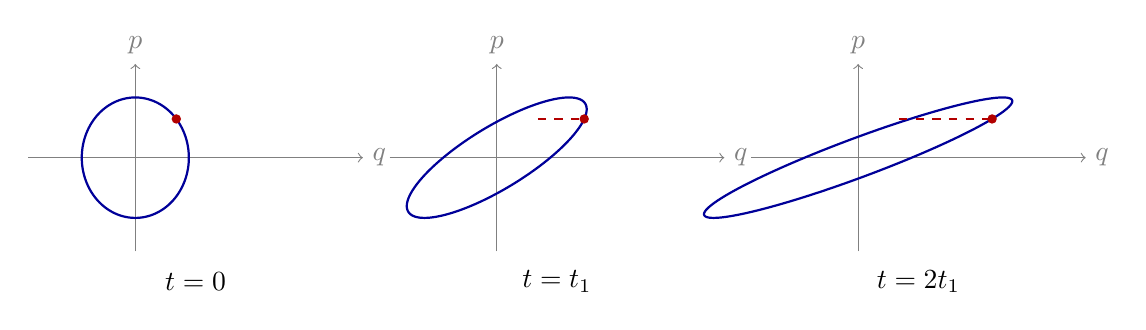
\begin{tikzpicture}[x=1cm,y=1cm,scale=0.85]
\def\ea{0.8}\def\eb{0.9}\def\thd{40}
\foreach \sh/\lab [count=\i from 0] in {0/{$t=0$}, 1.2/{$t=t_1$}, 2.4/{$t=2t_1$}}{
  \pgfmathsetmacro{\xs}{5.4*\i}
  \begin{scope}[xshift=\xs cm]
    \draw[->,gray] (-1.6,0) -- (3.4,0) node[right]{$q$};
    \draw[->,gray] (0,-1.4) -- (0,1.4) node[above]{$p$};
    \draw[thick,blue!60!black] plot[domain=0:360,samples=145,variable=\t]
         ({\ea*cos(\t)+\sh*\eb*sin(\t)},{\eb*sin(\t)});
    \pgfmathsetmacro{\px}{\ea*cos(\thd)+\sh*\eb*sin(\thd)}
    \pgfmathsetmacro{\py}{\eb*sin(\thd)}
    \pgfmathsetmacro{\pxz}{\ea*cos(\thd)}
    \draw[dashed,red!70!black] (\pxz,\py) -- (\px,\py);
    \fill[red!70!black] (\px,\py) circle (2pt);
    \node at (0.9,-1.85) {\lab};
  \end{scope}
}
\end{tikzpicture}
\caption{Free particle in the $(q,p)$ plane. The blue curve is a contour of a Gaussian mixed state; the red dot is one pure state in the ensemble that makes it up. The pure state moves along $p=\mathrm{const}$ (dashed). The mixed state is sheared: it elongates and tilts but its area, and with it the Gibbs entropy, is unchanged. Units are chosen so that the shear between panels is $t_1/m$.}
\label{fig:free}
\end{figure}

\subsection{The harmonic oscillator and the first anharmonic correction}

For $H=p^2/2m+m\omega^2q^2/2$ introduce $u_1=\sqrt{m\omega}\,q$ and $u_2=p/\sqrt{m\omega}$, so that $H=\omega(u_1^2+u_2^2)/2$ and the flow is a rigid rotation, $u_1(t)=u_1\cos\omega t+u_2\sin\omega t$, $u_2(t)=-u_1\sin\omega t+u_2\cos\omega t$. A Gaussian state with covariance $\Sigma_u$ rotates rigidly, and
\begin{equation}
\Var q(t)=\frac1{m\omega}\left[\frac{a+b}2+\frac{a-b}2\cos2\omega t+c\,\sin2\omega t\right],\qquad
a=\Sigma_{u,11},\ b=\Sigma_{u,22},\ c=\Sigma_{u,12}.
\end{equation}
The width oscillates at \emph{twice} the oscillator frequency. A state with $\Sigma_u=s\,\mathbb 1$ is invariant under rotations, hence stationary: it is the canonical state of Section~\ref{sec:bayes} with $s=\kB T/\omega$. The mean $(\Ave q,\Ave p)$ follows the classical orbit exactly, in accordance with Proposition~\ref{prop:mean}.

This changes when the potential is not quadratic. For $V(q)=\tfrac13\lambda q^3$, Eq.~\eqref{eq:meancorr} is exact, since $V'=\lambda q^2$ and $\Ave{q^2}=\Ave q^2+\sigma_q^2$:
\begin{equation}
m\,\frac{\dd^2\Ave q}{\dd t^2}=-\lambda\bigl(\Ave q^{\,2}+\sigma_q^2\bigr).
\end{equation}
A state centred on the equilibrium position $\Ave q=0$ nevertheless feels a net force $-\lambda\sigma_q^2$, which no pure state centred there would feel. The pure-state trajectory is the $\sigma_q\to0$ limit, and the formula says how fast the statistical description departs from it as the width grows.

\subsection{Chaos: how long does a state stay effectively pure?}
\label{sec:chaos}

Let the dynamics be chaotic with largest Lyapunov exponent $\lambda>0$. Two nearby pure states separate as $\delta(t)\approx\delta_0\eu^{\lambda t}$. If an observation leaves a state of width $w_0$ in phase space, its width grows as $w(t)\approx w_0\eu^{\lambda t}$ until it is comparable to the size $L$ of the region the system can explore. After that time,
\begin{equation}
t_*\simeq\frac1\lambda\ln\frac L{w_0},
\label{eq:predictability}
\end{equation}
the state cannot be treated as effectively pure, and only statistical statements about it are meaningful.

Equation \eqref{eq:predictability} has a logarithm, which makes the practical value of better data modest. Improving the initial precision by a factor of $10^6$ adds only $\lambda^{-1}\ln10^6\approx14\,\lambda^{-1}$ to the horizon. For the inner planets of the Solar System $\lambda^{-1}$ is of the order of a few million years \cite{Laskar1989}, so even a vast improvement in the data extends the horizon by a few tens of millions of years. Beyond it, the trajectory of the idealized pure state still exists as a mathematical object; what disappears is any real-world means of checking it. This is a concrete instance of the border between the ideal and the real world: predictions about the pure state at times $t\gg t_*$ are statements of the ideal world that no data can support.

\subsection{Many particles: from micro-sharp to macro-sharp}
\label{sec:manyparticles}

Take $N$ non-interacting point particles in the canonical state. The phase space has dimension $6N$, and in a pure state every observable has a sharp value, in particular every single-particle momentum. In the canonical state the opposite is true for a single particle: its momentum has the Maxwell distribution and is far from sharp. But consider a \emph{macroscopic} observable such as the total energy $E=\sum_{i=1}^{3N}\epsilon_i$, a sum of $3N$ independent quadratic terms. Each term has mean $\kB T/2$ and variance $(\kB T)^2/2$, so
\begin{equation}
\frac{\Var E}{\Ave E^2}=\frac{3N(\kB T)^2/2}{\bigl(3N\kB T/2\bigr)^2}=\frac{2}{3N},\qquad
\frac{\Delta E}{\Ave E}=\sqrt{\frac2{3N}}.
\end{equation}
\begin{center}
\begin{tabular}{r|cccc}
$N$ & $1$ & $10^3$ & $10^6$ & $10^{23}$\\ \hline
$\Delta E/\Ave E$ & $0.82$ & $2.6\times10^{-2}$ & $8.2\times10^{-4}$ & $2.6\times10^{-12}$
\end{tabular}
\end{center}
For macroscopic $N$ the mixed state makes the macroscopic observable \emph{sharp}, to a precision beyond any experiment, even though the same state is broad for individual molecules.

This allows us to state exactly what the traditional division by particle number does and does not capture. Both descriptions are ``deterministic'' at the level where they make sharp predictions. A pure state makes all observables sharp, in particular the microscopic ones. A canonical state of a large system makes the macroscopic observables sharp, with fluctuations of relative size $N^{-1/2}$. The thermodynamic limit $N\to\infty$ makes this sharpness exact. It is a second ideal-world limit, parallel to the pure-state limit $w_0\to0$ but taken at the macroscopic level: the pure state is the limit of infinite resolution, the thermodynamic limit is the limit of infinitely many degrees of freedom. The folklore that statistical mechanics is the theory of many particles arises because the second limit is reachable in practice when $N$ is large, while the first is never reachable. It does not follow that the two theories differ in kind.

\paragraph{Molecular dynamics as a numerical illustration.} A molecular-dynamics computation of an equilibrium average is an explicit implementation of the decomposition $\mu=\int\delta_z\,\dd\mu(z)$:
\begin{equation}
\Ave{A}_{\mu_t}=\int A\bigl(\varphi_t(z)\bigr)\,\dd\mu_0(z)\;\approx\;\frac1M\sum_{m=1}^{M}A\bigl(\varphi_t(z_m)\bigr),\qquad z_m\sim\mu_0.
\end{equation}
The outer loop draws initial conditions from the mixed state (the Maxwell--Boltzmann distribution for velocities, say), a Monte Carlo step. The inner computation integrates Hamilton's equations for each sample, that is, mechanics proper. The practice of computational physics uses the two sectors of the theory in exactly the division of labour described in this chapter.

% ---------------------------------------------------------------------
\section{Subsystems and the quantum case}
\label{sec:subsystems}

\subsection{Marginals: classically, pure wholes have pure parts}

Let the system consist of two parts $A$ and $B$ with phase space $\Gamma=\Gamma_A\times\Gamma_B$. The state of $A$ alone is the \emph{marginal} $\mu_A(X)=\mu(X\times\Gamma_B)$.

\begin{proposition}\label{prop:marginals}
A state $\mu$ on $\Gamma_A\times\Gamma_B$ is pure if and only if both marginals $\mu_A$ and $\mu_B$ are pure.
\end{proposition}

\begin{proof}
If $\mu=\delta_{(a,b)}$ the marginals are $\delta_a$ and $\delta_b$. Conversely, if $\mu_A=\delta_a$ and $\mu_B=\delta_b$, then $\mu\bigl(\Gamma\setminus\{(a,b)\}\bigr)\le\mu_A(\Gamma_A\setminus\{a\})+\mu_B(\Gamma_B\setminus\{b\})=0$.
\end{proof}

So classically a mixed state of a part is \emph{always} the consequence of an incomplete description of the whole. There is no mixedness that arises from the mere fact that a subsystem is a subsystem. A Brownian particle is described by a mixed state because the pure state of the fluid around it is not known; if it were known, the particle would follow a deterministic trajectory, which however is not generated by the Hamiltonian of the particle alone. The effective stochastic equations of the particle follow from marginalizing, in the sense of Eq.~\eqref{eq:bayes} and Section~\ref{sec:dynamics}, over the unknown state of the bath.

\subsection{A glance at the quantum case}
\label{sec:quantum}

The vocabulary of this chapter carries over to quantum mechanics, and it is instructive to see where it stops working. A quantum state is a density operator $\hat\rho\ge0$ with $\Tr\hat\rho=1$; the set of states is convex; the extreme points are the projectors $\hat\rho=|\psi\rangle\langle\psi|$, the \emph{pure states}; the law of motion is the von Neumann equation $\mathrm i\hbar\,\partial_t\hat\rho=[\hat H,\hat\rho]$, which maps pure states to pure states. So the architecture is the same: ``quantum mechanics'' is the pure-state sector of quantum statistical mechanics, and the entropy $-\kB\Tr\hat\rho\ln\hat\rho$ is zero for pure states, so that the $-\infty$ of the classical case is cut off at the quantum level, where the phase space has a natural cell of volume $h^n$.

Three differences prevent the classical ignorance reading from being carried over unchanged.
\begin{enumerate}[nosep]
\item Quantum pure states are not dispersion-free. No state gives all observables sharp values, so (b) of Proposition~\ref{prop:pure} fails for every state, and a pure state still yields probabilistic predictions.
\item The decomposition of a mixed state into pure states is not unique: the same $\hat\rho$ arises from many different ensembles of pure states. One cannot say that the system is ``really'' in one of the pure states of the mixture.
\item Proposition~\ref{prop:marginals} fails. A pure entangled state of two subsystems has mixed marginals, a mixedness that is not due to ignorance about anything.
\end{enumerate}
The pure/mixed distinction therefore remains meaningful in quantum theory, as the distinction between maximal and non-maximal information compatible with the theory, but ``mixed means ignorance'' is only partly true there. The chapter makes no claim to derive quantum mechanics; the claim is that classical mechanics and classical statistical mechanics are a single theory.

% ---------------------------------------------------------------------
\section{Objections and limits}
\label{sec:objections}

\paragraph{Does temperature depend on what I know?} In the maximum-entropy construction $\beta$ is the Lagrange multiplier that enforces a measured mean energy. Two observers with different data assign different states to the same system, and may make different predictions. This is not a defect but the normal behaviour of conditional probability, and it is adjudicated by experiment: the observer with better data makes sharper predictions that are still correct. For the macroscopic variables of a large system all reasonable observers agree up to $N^{-1/2}$ (Section~\ref{sec:manyparticles}), and this is why temperature appears as a property of the body.

\paragraph{Is an ensemble not simply a collection of physical copies?} Gibbs's ensemble can be read as relative frequencies in an actual or imagined collection of systems. The mathematics is identical, and claim (M) does not depend on the choice. The Bayesian reading is preferable when the system is unique (the Solar System, the Universe), because then there are no copies to count.

\paragraph{Is ergodicity not needed?} Ergodic theory enters when one wants to identify an ensemble average with the time average actually measured on a single system. In the Bayesian view the state \eqref{eq:maxent} is justified by the information, not by the dynamics; whether it predicts a measured time average then depends on the dynamics and on $N$. Whether this is a sufficient foundation is a matter of dispute: some authors regard the Bayesian justification as insufficient and prefer the Boltzmannian approach based on typicality.

\paragraph{Is the point $z^*$ real?} The classical ideal-world model says that the system has an exact phase point. Nothing in the real world can confirm this to arbitrary precision (Section~\ref{sec:bayes}). The Bayesian machinery can be used without asserting that $z^*$ exists; it plays the role of a regulative ideal, the limit towards which better data would move the state. In quantum mechanics this assumption fails altogether, as seen above.

% ---------------------------------------------------------------------
\section{Summary}

\begin{itemize}[nosep]
\item Mechanics and statistical mechanics share the phase space, the observables and the law of motion. They differ in the states they admit: points for mechanics, probability measures for statistical mechanics.
\item Pure states are characterized equivalently by being points, by being dispersion-free, by being multiplicative, and by being extreme in the convex set of states (Proposition~\ref{prop:pure}).
\item The Liouville equation maps pure states to pure states along Hamiltonian trajectories. Hamilton's equations are its characteristics, and mechanics is a closed subtheory (Proposition~\ref{prop:pure-stays-pure}).
\item In the Bayesian reading a mixed state quantifies incomplete knowledge. A pure state requires infinite information and is an ideal-world limit; real states are mixed. Updating and dynamics are different operations.
\item Hamiltonian evolution conserves the Gibbs entropy. The growth of entropy in the second law comes from coarse graining, that is, from the finite resolution of the observer.
\item The number of particles is not what separates the theories. Large $N$ makes macroscopic observables sharp in a mixed state, a second ideal limit that is attainable in practice.
\item Classically, mixedness is always ignorance (Proposition~\ref{prop:marginals}); in quantum theory it is not, although the pure/mixed vocabulary survives.
\end{itemize}

% ---------------------------------------------------------------------
\section*{Exercises}
\addcontentsline{toc}{section}{Exercises}

\begin{exercise}
Let $H=\tfrac12 z^{\mathsf T}Az$ with $A$ a symmetric $2n\times2n$ matrix. Show that a Gaussian state with covariance $\Sigma_0$ evolves into a Gaussian with $\Sigma_t=\eu^{tJA}\Sigma_0\,\eu^{tA J^{\mathsf T}}$ and constant $\det\Sigma_t$, and that the mean obeys $\dot{\Ave z}=JA\Ave z$. Specialize to the free particle and the oscillator.
\end{exercise}

\begin{exercise}
For the canonical state of one oscillator, with $h=2\pi\hbar$, show that $S=\kB\bigl(1+\ln(\kB T/\hbar\omega)\bigr)$. What happens as $T\to0$, and what does this say about the classical third law?
\end{exercise}

\begin{exercise}
Using Eq.~\eqref{eq:maxent}, derive the Maxwell distribution of the momentum of a single particle from the constraint $\Ave{p^2/2m}=\tfrac32\kB T$ in three dimensions. Which role does $N$ play in the derivation?
\end{exercise}

\begin{exercise}
Let $n=1$ and $V(q)=\tfrac13\lambda q^3$ (as in Section~\ref{sec:examples}). Initially $\Ave q=\Ave p=0$ and the state is Gaussian with $\sigma_q,\sigma_p>0$. Show that $\Ave q_t$ is not identically zero and compute its leading behaviour for small $t$. Compare it with the trajectory of the pure state at the same point.
\end{exercise}

\begin{exercise}
Prove Proposition~\ref{prop:marginals} in the other direction, that the marginals of a pure state are pure. Then construct a mixed state of two particles whose marginals are both pure. Why is it impossible? Compare with the quantum Bell state, whose marginals are maximally mixed.
\end{exercise}

\begin{exercise}
For a map or flow of your choice with a positive Lyapunov exponent, take $M=10^4$ initial conditions from a narrow Gaussian and propagate them numerically. Plot the width of the cloud against time and compare with Eq.~\eqref{eq:predictability}. Repeat with a cloud ten times narrower and check that the horizon grows by $\lambda^{-1}\ln10$.
\end{exercise}

% ---------------------------------------------------------------------
\section*{Notes and further reading}
\addcontentsline{toc}{section}{Notes and further reading}

The classical statement that the probability density is transported by Hamiltonian flow goes back to Gibbs \cite{Gibbs1902}. The embedding of nonlinear Hamiltonian flows into a linear theory of observables is due to Koopman \cite{Koopman1931}. The identification of statistical mechanics with inference under constraints, and the derivation of the canonical ensemble from the maximum-entropy principle, are due to Jaynes \cite{Jaynes1957}; its logical foundations, going back to Cox \cite{Cox1946}, are given in \cite{Jaynes2003}. Jaynes also stressed that entropy is a property of the description, not of the system alone \cite{Jaynes1965}. For an account of irreversibility from the Boltzmannian viewpoint see \cite{Lebowitz1993}; the geometrical formulation of mechanics used here is in \cite{Arnold1989}, and equilibrium statistical mechanics is covered in \cite{LandauLifshitz}.

\begin{thebibliography}{99}
\bibitem{Arnold1989} V.~I. Arnold, \emph{Mathematical Methods of Classical Mechanics}, 2nd ed., Springer, 1989.
\bibitem{Cox1946} R.~T. Cox, Probability, frequency and reasonable expectation, \emph{Am. J. Phys.} \textbf{14}, 1 (1946).
\bibitem{Gibbs1902} J.~W. Gibbs, \emph{Elementary Principles in Statistical Mechanics}, Scribner, 1902.
\bibitem{Jaynes1957} E.~T. Jaynes, Information theory and statistical mechanics, \emph{Phys. Rev.} \textbf{106}, 620 (1957); II, \textbf{108}, 171 (1957).
\bibitem{Jaynes1965} E.~T. Jaynes, Gibbs vs Boltzmann entropies, \emph{Am. J. Phys.} \textbf{33}, 391 (1965).
\bibitem{Jaynes2003} E.~T. Jaynes, \emph{Probability Theory: The Logic of Science}, Cambridge University Press, 2003.
\bibitem{Koopman1931} B.~O. Koopman, Hamiltonian systems and transformations in Hilbert space, \emph{Proc. Natl. Acad. Sci. USA} \textbf{17}, 315 (1931).
\bibitem{Laskar1989} J. Laskar, A numerical experiment on the chaotic behaviour of the Solar System, \emph{Nature} \textbf{338}, 237 (1989).
\bibitem{LandauLifshitz} L.~D. Landau and E.~M. Lifshitz, \emph{Statistical Physics, Part 1}, 3rd ed., Pergamon, 1980.
\bibitem{Lebowitz1993} J.~L. Lebowitz, Boltzmann's entropy and time's arrow, \emph{Physics Today} \textbf{46}(9), 32 (1993).
\end{thebibliography}
%%% END CHAPTER

\end{document}
